% !TeX root = ./2-handout.tex

%%Bonus slides on initial ordinals, continuum hypothesis, burali-forti (still need to finish the proper class stuff), and connectoins to axiom of choice are at the end commented out!
%also note that i didn't actually really get to discuss neo-logicism. so a bunch of the slides after prompt 4 are things we did not actually go over, but i've kept in as bonus stuff! 

% % Game plan: fill in some details from the summary handout for this week, especially relevant to solving problems

% Intersperse some practice problems, saving other ones for killing time

% Try to get to Frege by around 30 minutes in, or could end w/ this stuff? e.g. go through content and then in last 15 minutes fast forward to Frege no matter where. talk through for 7minutes and then the question?  

%lectures this week brought to by: https://www.youtube.com/watch?v=Uj3uJp6DK5k

%details on counters; setting it to 0 prints everything with a roman I
%https://www.overleaf.com/learn/latex/Counters

%https://tex.stackexchange.com/questions/555149/how-do-i-change-the-frame-continuation-counter-from-roman-numerals-i-ii-iii

% They could incorporate/do if needing to kill time:
% chalk and talk the review sheet for this week
% talk about the strangeness of reductio proofs (could do this in future as well!); but defs relevant this week given large number of reductio proofs on the pset 
%changes to notion of rigor in mathematics; e.g. bolzano moving away from physical intuition , motion, passage of time. 


%\newcounter{mysection}
%\setcounter{mysection}{1}
%\arabic{mysection}
%\roman{subsection}

%\begin{itemize}[<+->] 
%\item<2-> % reveals second and keeps on page in subsequent frames
%\begin{itemize}[<2->] %does for a whole list of items


\setcounter{section}{1} %sets section counter to 0. note that need to switch section counter from Roman to arabic for this to work! since no roman numeral for 0! %put this into preamble, i.e. file common.tex: \renewcommand\thesection{\arabic{section}}




\section{The Higher Infinite}
%\subsection*{test}

\begin{frame}
%\large

\scriptsize{\tableofcontents}

\end{frame}


\begin{frame}
\frametitle{Things Hunt is liable to forget to mention}
%\large

\begin{itemize}[<+->]


\item If you are on the waitlist and in class today, please let Hunt know after class and write your email (legibly) 

\item This Friday(!) is Minor completion date. Deadline for submission of Minor Completion Form for final-term seniors to avoid \$50 fee! 
\item[] Don't give The Corporation your hard-earned dolla dolla bills!!!! 

\item Feel free to join \href{https://piazza.com/mit/spring2023/24118}{Piazza}! 

\item Feel free to join PSet partners!!! 
\item[] Groups will be auto-assigned Friday

%\item If you haven't yet, please complete the Most Basic Factz survey on Canvas
%\item[] Attendance for last Tuesday 2/7/23

\item This week's office hours (metaphysics is CANCELED): \\ today, 12--12:55 \& 2:10--3

\item PSet 2 will be posted by Friday; due Sunday March 5th! \\ (sounds further away b/c February is the SHORTEST month)



\end{itemize}
\end{frame}

\subsection{Ducks in a Row}

\begin{frame}
\frametitle{The BIG Picture}
%\large

\begin{itemize}[<+->]

\item For no other reason than because we can (allegedly), our goal is to construct sets of larger and larger cardinality

\item To do so, we rely on a distinct kind of `number' known as \textit{ordinals}

\item As the name suggests, ordinals arise from the study of orderings

\item Just as cardinalities represent isomorphisms for the purposes of counting, ordinals represent isomorphisms for the purposes of ordering elements in a series. 

\item Of course, these mega-large numbers are interesting perhaps insofar as we have reason to believe they exist, so we'll take some excursions into the ontological status of numbers

\end{itemize}
\end{frame}

\begin{frame}
\frametitle{Strict Orderings}
%\large

\begin{itemize}[<+->]

\item \emph{Strict Ordering}: a relation $<$ constitutes a strict ordering on a set $S$ just in case it satisfies the following two conditions:

\begin{enumerate}

\item[] For any a, b, and c in $S$, we have

\item \textbf{Asymmetry}: If $a < b$, then it is not the case that $b < a$

\item \textbf{Transitivity}: If $a < b $ and $b < c$, then $a < c$

\end{enumerate}

\bigskip 

\item Note that asymmetry entails irreflexivity: $\forall a \in S$, $\enot (a < a)$

\item Concept of `strict ordering' captures our intuitive notion of precedence, i.e. of what it is for one thing to precede another
% you might even think that these conditions are constitutive of the meaning of precedence

\end{itemize}
\end{frame}

\begin{frame}
\frametitle{Strict Total Orderings}
%\large

\begin{itemize}[<+->]

\item A \emph{strict total ordering} is a strict ordering that is also total:

\item \textbf{Totality}: $\forall a, b \in S$ such that $a \neq b$, either $a < b$ or $b < a$ \\ (and by asymmetry, this is an exclusive-or for strict orderings)

\end{itemize}
\end{frame}

\begin{frame}
\frametitle{``How would you like that?" Well-ordered plz}
%\large

\begin{itemize}[<+->]

\item A \emph{well-ordering} is a strict total ordering such that: 

\item Every non-empty subset has a smallest member according to the ordering

\item[] -- i.e. $\forall$ non-empty subsets $S$, $\exists$ some $s \in S$ such that $s < y$ for every other $y \in S, y \neq s$

% Note that if the set was not strictly ordered, we could have ties, i.e. two elements that are the `smallest'. And presumably that would mess some stuff up?

% Question: does a well-ordering have to be strict?
%This fact seems to indicate yes: ``Every element s of a well-ordered set, except a possible greatest element, has a unique successor (next element), namely the least element of the subset of all elements greater than s. " So this seems to rule out a tree structure. 

\item To show a set is not a well-ordering, it suffices to:

\item[1.)] show it is not a strict total order or

\item[2.)] show that there exists a subset that does not have a unique smallest member according to the ordering

% % I guess a nice little homework problem would have been the following: show that the smallest member in a subset of a well-ordered set is unique. Proof: by definition, the smallest member is less than every other member in the subset. By asymmetry, this means that no other member is less than this smallest member. so no other member can be the smallest member. 

%interesting feature which is not intuitive to me: ``There may be elements besides the least element which have no predecessor"
%example: \omega + \omega (e.g. by doing the evens, then doing the odds). In this case, neither 0 nor 1 have predecessors! 

\end{itemize}
\end{frame}

\begin{frame}
\frametitle{Some Practice with Strict Total-Orderings}
%\large


Which of the following sets are strictly totally ordered by the defined relation `$<$'? If not, provide a concrete counterexample! \\

Remember to check: (i) asymmetry, (ii) transitivity, and (iii) totality

\begin{enumerate}[<+->]

\item The set of natural numbers, where $1 < 2 <3 < \dots < 0$?
% % Clearly transitive, clearly asymmetric, and clearly total.

\item The set of rationals, where $a < b$ iff $b = a + q$ for some $q \in \mathbb{Q}^{>0}$
% yes, note that for any two distinct arbitrary rational numbers, one of them is at least $q$-greater than the other. Note that if we allow $q=0$, then we would not have a strict ordering because every rational would then relate to itself! so we'd have reflexivity

\item Same as above but we allow $q=0$? 

\item The set $\mathcal{P}(\{ 0, 1, 2, 3 \})$, where $a < b$ iff $a \subsetneq b$
% note that to solve this problem, you don't actually need to explicitly write down the 16 members in the power set. It suffices to notice that $\{ 0 \}$ and $\{1 \}$ are both in the power set, but neither is a proper subset of the other, so neither $0 < 1 $ nor $1 < 0$, so this is not a TOTAL order. 

\item The set of Olympic athletes, where $a < b $ iff $a$ has won fewer medals than $b$
% no: there exist Olympic athletes who have won the same number of medals, in which case neither precedes the other. Technically, I should provide a concrete counterexample. 
%both Ryan Lochte and Natalie Coughlin have won 12 medals in US swimming. 

\item The set of people on Earth, where $a < b$ iff $a$'s birth-year precede's $b$'s birth-year
% not a total order because some people were born in the same year

% Copying problem 6 from the MITx. At least 5 problems to copy over!

% Clarify difference between strict vs. non-strict total ordering (irreflexive vs. reflexive)


\end{enumerate}
\end{frame}

\begin{frame}
\frametitle{Some Practice with Well-orderings}
%\large

\begin{itemize}[<+->]

\item Notation: distinguish phi-symbol `$\phi$' from the empty set `$\emptyset$'

\item Is $\powerset(\emptyset)$ well-ordered by $\in$?
%yes it is, trivially! 

\item Is $\powerset(\mathbb{Q})$  well-ordered by $\subseteq$?
% No, it is not even a total ordering. Note that $\powerset(\mathbb{Q})$ contains $\{ 5 \}$ and $\{ 1/2 \}$, but neither is a subset of the other.

\item What is $\powerset^3(\emptyset) := \powerset (\powerset (\powerset (\emptyset))) $? 

\end{itemize}
\end{frame}

\begin{frame}
\frametitle{A Gloss on Ordinals}
%\large

\begin{itemize}[<+->]

\item We can characterize well-orderings up to isomorphism (depicted diagrammatically with our friendly tally mark notation) 

\item \emph{Isomorphism between well-orders}: consider two well-ordered sets $A$ and $B$ with the orderings $<_1$ and $<_2$, respectively. \\ Ordering $(A, <_1)$ is isomorphic to ordering $(B, <_2)$ just in case:

\begin{enumerate}

\item There exists a bijection $f$ between sets $A$ and $B$

\item $\forall x, y \in A$, $x <_1 y$ iff $f(x) <_2 f(y)$

\end{enumerate}

\bigskip

\item Ordinals are sets that represent these well-ordering types. \\ Each distinct ordinal represents a distinct kind of well-ordering 


\end{itemize}
\end{frame}




\subsection{Frege's Conception of Number}
% I'm drawing heavily on Shapiro's discussion in chapter 6 (logicism) of thinking about mathematics. Probably some better discussions of this stuff.

% Given that this course descends from George Boolos, it would be interesting to discuss his criticisms of neo-logicism, e.g. 1997 arguing against Wright's appeal to concept formation by abstraction.

\begin{frame}
\frametitle{Hume's Principle}
%\large

% % Interesting that part of Frege's motivation was to define the cardinal numbers independently of the ordinal numbers. Whereas Cantor had used the ordinal numbers to define the cardinal numbers. I should probably look into the history of what Cantor was doing, since it might help motivate studying the ordinals. Maybe this is related to using the ordinals as blueprints to define sets of higher cardinality.

\begin{itemize}[<+->]

\item \emph{Hume's Principle}: for any concepts $F, G,$ the number of $F $ is identical to the number of $G $ if and only if $F$ and $G$ are equinumerous
% idea described on page 134 of Shapiro: the left hand side of the HP has a grammatical form involving objects. The right hand side supplies truth conditions, which we then use to show the existence of these objects.

\item `equinumerous' means ``same cardinality," i.e. there exists a bijection between the objects that fall under each concept 

\item Obviously, to use HP to \textit{define} numbers, we have to define `equinumerous' in a way that doesn't refer to numbers

\item Frege showed how to do this using (2nd-order) logic alone
% % i should probalby know how this is done haha! 

%second-order logic (where you can quantify over properties)



\end{itemize}
\end{frame}

\begin{frame}
\frametitle{Getting Ontology out of Hume's Principle}
%\large

\begin{itemize}[<+->]

\item \emph{Hume's Principle}: for any concepts $F, G,$ the number of $F $ is identical to the number of $G $ if and only if $F$ and $G$ are equinumerous

\item We interpret `the number of $F$' as being a name of an \textit{object}, what logicians call a `singular term'. 
\item[] It is just like a definite description such as ``the author of \textit{The Audacity of Hope}"

\item This interpretation will matter for a logicist recovery of \textit{realism in mathematical ontology}, a form of Platonism. 

\item As in: I see dead people. Frege saw numbers. 

\end{itemize}
\end{frame}

\begin{frame}
\frametitle{Frege's Conception of Numbers: Getting Started}
%\large

\begin{itemize}[<+->]

\item Consider the concept \textsc{not identical to itself}; represented by a predicate $Z$

\item Notice that every object is identical with itself \\ (indeed, this might be a paradigmatic law of logic!)

\item Hence, no object has the concept \textsc{not identical to itself}: this concept has empty \textit{extension} (i.e. for all objects $c$, $Zc$ is false)

\item Define the number zero to be \textit{the number of the concept} \\ \textsc{not identical to itself}

\item Notice that this definition is (i) a priori (no empirical knowledge involved) and (ii) stance-independent (does not depend on attitudes of people)

\end{itemize}
\end{frame}

\begin{frame}
\frametitle{Frege's conception of numbers: just keep going!}
%\large

\begin{itemize}[<+->]

\item Define the \#1 to be the number of the concept \textsc{identical to zero}

\item Define the number 2 to be the number of the concept \\ \textsc{either identical to zero or identical to one}, etc.

\item HP implies that each of these natural numbers are distinct 
%different from each other

\item Hence, HP is true only if there are infinitely-many objects! 
\item[] -- So commitment to HP entails commitment to an actual infinity of objects! (So I guess I'm buying a mac!)
% This is similar to a kind of proof we did at the end of logic class! Showing that certain claims could not be true in models with only finitely-many objects

\item One can define a successor function on the numbers and derive the basic principles of arithmetic from Hume's principle

\end{itemize}
\end{frame}

\begin{frame}
\frametitle{Deriving $0=0$}
%\large

\begin{itemize}%[<+->]

\item Logical truth: the concept of `not identical to itself' is equinumerous with the concept `not identical to itself'

\item Hume's principle $\Rightarrow$ the number of non-self-identical things is identical to the number of non-self-identical things

\item Let the symbol `0' denote the number of non-self-identical things

\item Conclusions: $0=0$, so it appears that zero exists. 

\end{itemize}
\end{frame}

\begin{frame}
\frametitle{On the Epistemic Status of Hume's Principle}
%\large

\begin{itemize}[<+->]



\item Is Hume's principle part of `logic'?

\item Hume's principle is not a tautology (so it is not true in virtue of form alone)

\item As far as we know, no canonical laws of logic entail Hume's principle (e.g. laws like $\enot(P \eand \enot P)$ )
% law of non-contradiction
% % what are some examples of canonical laws of logic? I guess I should really have these kinds of things in mind?

\end{itemize}
\end{frame}

%%%note that I have commented out the slides I didn't get to on 2-23-23, but left them in order, since if I use these again for a future phil math class, I'd prefer to keep the original order. But moving them to after the prompt for now! 
\iffalse %**********************************************************************************************************

\begin{frame}
\frametitle{Frege's foibles}
%\large

\begin{itemize}[<+->]

\item Frege aimed to \textit{derive} Hume's principle from principles that seem genuinely logical in nature

\item One of these is his ``Basic Law V'', which Russell (and earlier Zermelo) showed to be inconsistent (Russell's paradox). 
% Ironically, Russell ultimately rejected this immediate upshot of's paradox, arguing instead that the resulting argument against Frege is fallacious because it it relies on impredicative definition, and Russell and Whitehead aimed to ban impredicative definitions on the grounds that they are viciously circular
% good example of an impredicative definition given by Shapiro: least upper bound is defined impredicatively: the smallest number in the set of upper bounds. So in defining `least upper bound', we refer to the set of upper bounds, of which the least upper bound is a member. According to Shapiro, many mathematical concepts seemingly require impredicative definitions
% Russell and Whitehead ultimately introduce the axiom of reducibility as a way to make the use of impredicative definitions safe and avoid vicious circles. So that is a sense in which this axiom seems more ad hoc and less of a logical nature
% likewise for the axiom of infinity, which they needed to introduce to recover the natural numbers. Since they don't have Hume's principle, they are not able to derive the natural numbers. But on the same grounds, Hume's principle is basically a kind of axiom of infinity.

\item Neo-logicists today give up on deriving Hume's principle and take it as a starting point. 


\end{itemize}
\end{frame}



\begin{frame}
\frametitle{A Slide to Skip (some background)}
%\large

% % Note that Frege's basic law V is seemingly equivalent to the principle of unrestricted comprehension. ZF set theory has an axiom of restricted comprehension, commonly called axiom of separation. It says that given a set A and a predicate P, there is a subset of A that has property P. 

\begin{itemize}%[<+->]

\item Frege's Basic Law V: for any concepts F, G, the extension of F is identical to the extension of G iff for every object a, Fa iff Ga

\item Derivation of Russell's paradox relies on an impredicative definition (e.g. ``set of \textit{all sets} that do not contain themselves")

\item A definition is `impredicative' if it refers to a collection that contains the entity being defined

\item[] e.g. defining the `least upper bound' as the smallest of the upper bounds

\item Ironically, Russell argued for a ban on impredicative definitions, so he ultimately rejected the legitimacy of his namesake paradox (at least as an argument against Basic Law V)!

\item To avoid impredicative definitions (and the circularity they involve) Russell and Whitehead developed a (ramified) type theory 


\end{itemize}
\end{frame}

\begin{frame}
\frametitle{Of Numbers and Caesar}
%\large

\begin{itemize}[<+->]

\item Hume's principle only applies to identities that have the form \\ ``the number of $F$ $=$ the number of $G$"

\item What of identities of the form ``the number of $F = j$", where $j$ is some other name, e.g. a name of Josh$_2$? 

\item As far as HP is concerned, it may be the case that Josh$_2$ $= 118$.  

\item Or, more famously, Julius Caesar might equal the number $2 $

% Frege had a somewhat plausible response to this worry involving extensions. But the neo-logicist, such as Wright and Hale, avoid this response. So they have to go some other way. See Hale 1994. shapiro intro book, p. 137

\end{itemize}
\end{frame}

\fi %******

\begin{frame}
\frametitle{Philosophy Prompt \#4: what is the number of this prompt?}
%\large

\begin{itemize}[<+->]

\item What does it mean to say that this is the 4th philosophy prompt in this class? In other words, what is the number 4?

\item Alternative questions: how are you feeling about Hume's Principle? Is it a law of logic? Is it at least analytic? Or knowable a priori? 

\item \emph{Hume's Principle}: for any concepts $F, G,$ the number of $F $ is identical to the number of $G $ if and only if $F$ and $G$ are equinumerous

\end{itemize}
\end{frame}

%\iffalse %**********************************************************************************************************
\iffalse
\begin{frame}
\frametitle{Uniqueness of Zero?}
%\large

\begin{itemize}[<+->]

\item A natural question: how do we know that zero is unique?
% Indeed, Chloe asked this question on Thursday 2/22, 2023

\item For instance, in group theory, one proves that the identity element is unique. Assume that another identity element exists, and show that it must equal the first:
% 0 + 0' = 0  and 0+0' = 0', since both are units. So 0 = 0' 

\item In arithmetic, we seemingly need to prove that there is a unique initial object. 

%seemingly I could explain this by using Peano arithmetic axioms!
%see here: https://www.youtube.com/watch?v=3gBoP8jZ1Is
%key claim: the zero is never a successor of any other number! and we definte successor function as injective. 

%proof: assume there are two zeros 0 and 0'. then by injectivity of S, if S(0) = S(0') entails that 0 = 0'. worry: what is to prevent there as well from being two different 1's? e.g. s.t. S(0) = 1 whereas S(0') = 1' and 1 \neq 1'? 
%does axiom of induction somehow prevent this kind of non-standard model? 

%definition of natural numbers from peano arithmetic: the minimal, non-empty set that admits a successor function, where this function satisfies peano's five axioms. 
%note that addition and multiplication be defined using the successor function. 

%\item Does the following work: Assume for the sake of argument that there is another initial object 0'. Then its successor is also 1 (since we are recovering arithmetic, which has the well-ordering property). So then $0' = 0$

\end{itemize}
\end{frame}
\fi 

\begin{frame}
\frametitle{Frege's foibles}
%\large

\begin{itemize}[<+->]

\item Frege aimed to \textit{derive} Hume's principle from principles that seem genuinely logical in nature

\item One of these is his ``Basic Law V'', which Russell (and earlier Zermelo) showed to be inconsistent (Russell's paradox). 
% Ironically, Russell ultimately rejected this immediate upshot of's paradox, arguing instead that the resulting argument against Frege is fallacious because it it relies on impredicative definition, and Russell and Whitehead aimed to ban impredicative definitions on the grounds that they are viciously circular
% good example of an impredicative definition given by Shapiro: least upper bound is defined impredicatively: the smallest number in the set of upper bounds. So in defining `least upper bound', we refer to the set of upper bounds, of which the least upper bound is a member. According to Shapiro, many mathematical concepts seemingly require impredicative definitions
% Russell and Whitehead ultimately introduce the axiom of reducibility as a way to make the use of impredicative definitions safe and avoid vicious circles. So that is a sense in which this axiom seems more ad hoc and less of a logical nature
% likewise for the axiom of infinity, which they needed to introduce to recover the natural numbers. Since they don't have Hume's principle, they are not able to derive the natural numbers. But on the same grounds, Hume's principle is basically a kind of axiom of infinity.

\item Neo-logicists today give up on deriving Hume's principle and take it as a starting point. 


\end{itemize}
\end{frame}



\begin{frame}
\frametitle{A Slide to Skip (some background)}
%\large

% % Note that Frege's basic law V is seemingly equivalent to the principle of unrestricted comprehension. ZF set theory has an axiom of restricted comprehension, commonly called axiom of separation. It says that given a set A and a predicate P, there is a subset of A that has property P. 

\begin{itemize}%[<+->]

\item Frege's Basic Law V: for any concepts F, G, the extension of F is identical to the extension of G iff for every object a, Fa iff Ga

\item Derivation of Russell's paradox relies on an impredicative definition (e.g. ``set of \textit{all sets} that do not contain themselves")

\item A definition is `impredicative' if it refers to a collection that contains the entity being defined

\item[] e.g. defining the `least upper bound' as the smallest of the upper bounds

\item Ironically, Russell argued for a ban on impredicative definitions, so he ultimately rejected the legitimacy of his namesake paradox (at least as an argument against Basic Law V)!

\item To avoid impredicative definitions (and the circularity they involve) Russell and Whitehead developed a (ramified) type theory 


\end{itemize}
\end{frame}

\begin{frame}
\frametitle{Of Numbers and Caesar}
%\large

\begin{itemize}[<+->]

\item Hume's principle only applies to identities that have the form \\ ``the number of $F$ $=$ the number of $G$"

\item What of identities of the form ``the number of $F = j$", where $j$ is some other name, e.g. a name of Josh$_2$? 

\item As far as HP is concerned, it may be the case that Josh$_2$ $= 118$.  

\item Or, more famously, Julius Caesar might equal the number $2 $

% Frege had a somewhat plausible response to this worry involving extensions. But the neo-logicist, such as Wright and Hale, avoid this response. So they have to go some other way. See Hale 1994. shapiro intro book, p. 137

\end{itemize}
\end{frame}


\begin{frame}
\frametitle{What to make of Hume's Principle?}
%\large

\begin{itemize}[<+->]

\item Hume's principle is true only in infinite models.

\item Hence, commitment to Hume's principle entails commitment to an infinite number of objects in your domain of discourse
\item[] --In this sense, HP is equivalent to an ``axiom of infinity"

\item Provides a reason for thinking that Hume's principle cannot \textit{define} cardinal numbers, at least if you think that definitions should not entail the existence of objects

\item Nonetheless, one might argue that Hume's principle is \textit{part of the meaning} of the concept of \textit{natural number}

\item Hume's principle could then be a necessary, analytic feature of numbers, and knowable a priori

\end{itemize}
\end{frame}

\begin{frame}
\frametitle{Logicism today: Neo!}
%\large

\begin{itemize}[<+->]

\item \emph{Neo-logicism}: (i) we can know many mathematical truths \\ \textit{a priori}, deriving them from rules that are analytic or meaning-constitutive of the relevant mathematical concepts \\ (e.g. the concept \textsc{Number}) 
\item[] (ii) realism in ontology: objective, mind-independent mathematical objects exist
% % advantage of the root through logicism is to avoid some epistemic problems for Platonism otherwise construed. Mathematics becomes knowable a priori. We do not need causal connection with these abstract objects. We also do not need to appeal to some mysterious notion of intuition.

\item Using Hume's principle and second-order logic, one can derive the natural numbers and arithmetic (``Frege's theorem")
% % where Frege's original program goes wrong is that he aims to derive Hume's principle using the concept of extensions and the inconsistent Basic Law V. So Wright and Hale basically argue that they can recover Frege's program simply by starting with Hume's principle and second-order logic
% Shapiro notes that Hume's principle is consistent if (second-order) arithmetic is consistent.

\item Whether this shows arithmetic is epistemically closer to `logic' than `mathematics' depends on the status of 2nd-order logic

\item Quine: second-order logic is just disguised set theory \\ (`a wolf in sheep's clothing')
% C Quine 1986, philosophy of logic, second edition. Quoted by Schapiro on page 136. See especially chapter 5 of Quine.


\end{itemize}
\end{frame}





\subsection{Ordinal Arithmetic}


\begin{frame}
\frametitle{Why we care about Well-Orderings}
%\large

\begin{itemize}[<+->]

\item \textbf{Well-ordering theorem}: every set can be well-ordered

\item Ordinals are sets that represent all of the possible distinct kinds of well-orderings (distinct up to isomorphism)

\item The ordinals themselves are well-ordered by the set-membership relation $\in$

\item We can define arithmetic operations on ordinals, and use them to construct sets of extremely large cardinality

\end{itemize}
\end{frame}

\begin{frame}
\frametitle{The First Few Ordinals}
%\large

\[
\begin{array}{ccc}
\text{ordinal} & \text{name of ordinal} & \text{well-order type represented}\\ \hline
\set{} &0 & \ \\
\set{0} &0'  & |   \\
\set{0,0'} &0''  & | |  \\
\set{0,0',0''} &0''' & | | |  \\
\vdots  & \vdots\\
\set{0,0',0'',0''',\dots} &\omega  & | | |  \dots   \\
\set{0,0',0'',0''',\dots,\omega} &\omega'  & | |  | \dots |  \\
\set{0,0',0'',0''',\dots,\omega, \omega'} &\omega''  & | | | \dots | |  \\
\vdots & \vdots & \vdots \\
\end{array}
\]

\end{frame}

\begin{frame}
\frametitle{Ordering the Ordinals}
%\large

\begin{itemize}[<+->]

\item The ordinals are well-ordered by the following precedence relation:
$$\alpha <_o \beta \leftrightarrow_{\text{\emph{df}}} \alpha \in \beta$$

\item e.g. the ordinal named by $0''$ is $<_o$ the ordinal named by $0'''$ because $0'' \in 0''' = \{0, 0', 0'' \}$

\end{itemize}
\end{frame}

\begin{frame}
  \frametitle{Happy Belated Birthday to Brouwer yesterday!}

  \begin{columns}
    \begin{column}{.4\textwidth}
      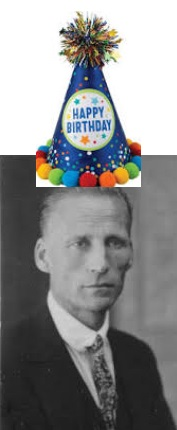
\includegraphics[height=.8\textheight]{../assets/Brouwer_hat}
    \end{column}
    \begin{column}{.6\textwidth}
      \begin{itemize}[<+->]
        \item L.E.J. Brouwer (27 Feb. 1881--1966)
        \item A founder of topology \\ (fixed-point theorem!)
        \item A mathematical iconoclast! \\ Foremost proponent of intuitionism
\item Bertus says, ``Math is in your MINDS y'all!'' 

%fixed point theorem basically says: if you lay a map of US over any part of US, there is some point of the map that is directly over the point of the US that it represents. 
%should do an excursion on intuitionism
%one on formalism
%and perhaps on Brouwer/Hilbert debate. Team Brouwer is heyting and weyl (hilbert student) vs. Hilbert, Bernays, Ackermann, and von Neumann 
      \end{itemize}
    \end{column}
  \end{columns}
\end{frame}



\begin{frame}
\frametitle{Ordinal Addition}
%\large

\begin{itemize}[<+->]

\item \emph{Addition Heuristic}: A well-ordering of type $(\alpha+\beta)$ is the result of starting with a well-ordering of type $\alpha$ and appending a well-ordering of type $\beta$ at the end.

\item Mnemonic: $\alpha +_o \beta$ wears this structure in its left to right order! 

\item Ordinal addition is associative: \((\alpha+\beta)+\gamma = \alpha+(\beta+\gamma)\).

\item Ordinal addition is \emph{not} commutative: \\ it is not generally the case that $\alpha + \beta = \beta + \alpha$.

\end{itemize}
\end{frame}


\begin{frame}
\frametitle{Practice with Ordinal Addition $+_o$}
%\large

Heuristic definition: $\alpha +_o \beta$ means (i) start with a well-ordering of type $\alpha$ and (ii) APPEND a w.o. of type $\beta$ at the end (i.e. to the right). 

Mnemonic: $\alpha +_o \beta$ wears this structure in its left to right order! 

\begin{enumerate}[<+->]

\item Does \(0' + 0''' = 0''' + 0'\)? 
% True. \(0' + 0''' = 0'''' = 0''' + 0'\)

\item Does \(0' + \omega = \omega' + 0\)? 
% False. \(0' + \omega = \omega\), but \(\omega' + 0\) is \(\omega'\).

\item Does \(0' + \omega = 0 + \omega'\)?
% false: \(0' + \omega = \omega\), but \(0 + \omega'\) is \(\omega'\)

\item Is \((\omega + 0'') + \omega <_o (\omega + \omega) + 0''\)? 
% True. \((\omega + 0'') + \omega = \omega + \omega\), which is smaller than \((\omega + \omega) + 0''\).

\item Does \(0' + \omega = \omega + 0'\)?
% False. \(0' + \omega = \omega\), but \(\omega + 0'\) is greater than \(\omega\).

\item Is $0'' + 0' <_o 0 + 0''' $? 
%False. \(0 + 0''' =  0''' = 0'' + 0'\).

\end{enumerate}
\end{frame}

\begin{frame}
\frametitle{Ordinal Multiplication}
%\large

\begin{itemize}[<+->]

\item \emph{Multiplication Heuristic}: A well-ordering of type $(\alpha\times\beta)$ is the result of starting with a well-ordering of type $\beta$ and replacing each position in the ordering with a well-ordering of type $\alpha$.

\item Mnemonic: we multiply $\alpha$ \textit{into} $\beta$, like distribution: $2 \times (5+7+47)$

\item Ordinal multiplication is associative: \((\alpha\times\beta)\times\gamma = \alpha\times(\beta\times\gamma)\).

\item Ordinal multiplication is \emph{not} commutative: \\ it is not generally the case that $\alpha \times \beta = \beta \times \alpha$.

\end{itemize}
\end{frame}

\begin{frame}
\frametitle{Practice with Ordinal Multiplication $\times_o$}
%\large
\bi

\item Heuristic: $\alpha \times_o \beta$ means (i) start with a well-ordering of type $\beta$ and (ii) REPLACE each position in this w.o. by a w.o. of type $\alpha$ 

\item Mnemonic: we multiply $\alpha$ \textit{into} $\beta$, like distribution: $2 \times (5+7+47)$
%$2 \times (50+9)$

\item Mnemonic: Try to be beta first\dots before going ALPHA! 
%Beta-males finish first (opposite of nice guys finish last). %be beta (like be better). Beta first; alpha second. 
%best starts with beta. best to start with beta. 
\ei

\begin{enumerate}[<+->]

\item Does \(0' \times 0''' = 0''' \times 0'\)? 
% True. 

\item Does $\omega \times 0'''$ = $0''' \times \omega$?
% False. $\omega \times 0''' = \omega + \omega + \omega$ but $0''' \times \omega = \omega$

\item Does \(0''' \times \omega = (\omega + \omega) + \omega\)?
%False.  \(0''' \times \omega = \omega\), which is smaller than \((\omega + \omega) + \omega\).

\item Does \(\omega \times 0''' = \omega + (\omega + \omega)\)?
%True. \(\omega \times 0''' = \omega + (\omega + \omega)\)

\item Is \(\omega \times \omega <_o \omega \times (0'' \times \omega)\)
% False. \(\omega \times (0'' \times \omega) = \omega \times \omega\).


\end{enumerate}
\end{frame}

\begin{frame}
\frametitle{Addition PLUS Multiplication???}
%\large
%both true 

\begin{enumerate}[<+->]

\item Is \((\omega \times 0'') + \omega <_o (\omega \times \omega) + 0''\)?
%True. \((\omega \times 0'') + \omega = ((\omega + \omega) + \omega)\), which is much smaller than \(\omega \times \omega\) (and therefore much smaller than \((\omega \times \omega) + 0''\).)

\item Does \(\omega \times (\omega + \omega) = (\omega \times \omega) + (\omega \times \omega)\)?
%True. \(\omega \times (\omega + \omega)\) is the result of using \((\omega + \omega)\) as a template, and filling each position with an \(\omega\)-sequence. So we get an \(\omega\)-sequence of \(\omega\)-sequences followed by an \(\omega\)-sequence of \(\omega\)-sequences. 
%Right hand side: \((\omega \times \omega) + (\omega \times \omega)\) is the result of starting with a sequence of type \((\omega \times \omega)\) (i.e. an \(\omega\)-sequence of \(\omega\)-sequences), and appending another sequence of type \((\omega \times \omega)\) (i.e. another \(\omega\)-sequence of \(\omega\)-sequences) to the right. So, again, we get an \(\omega\)-sequence of \(\omega\)-sequences followed by an \(\omega\)-sequence of \(\omega\)-sequences



%%practice with formal definiton of addition; could include if time:
%\item  \question{\(\alpha + 0' = \alpha \cup \{\alpha\}\) ($\alpha$ an ordinal)}

%\answer{True. It follows from the Construction Principle that \(\alpha \cup \{\alpha\} = \alpha'\), and it follows from the definition of addition that  \(\alpha + 0' = (\alpha + 0)' = \alpha'\). Putting the two together, \(\alpha \cup \{\alpha\} = \alpha'\) .}

\end{enumerate}
\end{frame}




\subsection{Benacerraf's Identification Problem}

\begin{frame}
\frametitle{Platonism: ontological realism}
%\large

\begin{itemize}[<+->]

\item \emph{Platonism}: some mathematical entities exist as abstract objects

\item What does it mean for an abstract object to exist?

\item Some standard criteria for (objective) abstract objects:

\bigskip

\begin{itemize}

\item \textbf{Mind-independent}: do not depend on features of agents, \\ e.g. consciousness

\item \textbf{Non-physical}: exist independently of physical reality, \\ e.g. `outside' the universe, beyond space--time

\item \textbf{Eternal}: possess immutable, intrinsic properties

\end{itemize}

\medskip

\item Understand `abstract' in contrast with `concrete'


\end{itemize}
\end{frame}

\begin{frame}
\frametitle{Set-theoretic Platonism: numbers as sets}
%\large

\begin{itemize}[<+->]
% historical question: when exactly did people figure out that most parts of mathematics could be modeled (or reduced to) set theory?

\item Seemingly all parts of mathematics can be modeled in set theory

\item Natural idea: take sets as supplying the basic kind of ontological entity for all other mathematical structures: \\ numbers, functions, points, spaces, etc.

\item \textbf{Set-theoretic Platonism}: math objects exist as abstract sets
%, possibly endowed with certain relations (where relations are themselves sets, e.g. defined on Cartesian products) 

\end{itemize}
\end{frame}

\begin{frame}
\frametitle{A Burden for Platonism}
%\large

\begin{itemize}[<+->]

\item Ideally, a Platonist ought to provide a criterion that determines whether any given mathematical object is identical or distinct with any other object (abstract or concrete)

\item Quine: ``No entity without identity''!

%As Quine said, ``No entity without identity''; quoted by shapiro (p. 112) neat how my indispensability paper basically shares this intuition, which I recall Alan Baker trying to reject in conversation. 

\item A Platonist ought to be able to tell us whether or not the number $4$ is distinct from Julius Caesar

\item e.g., with Hume's principle alone, Frege's conception of number does not determine whether the following statement is true or false: `$ 4 = $ Julius Caesar'

\item As far as HP is concerned, the number of the concept ``\textsc{identical to 0 or 1 or 2 or 3}'' might just be Julius Caesar
% recall on the further account that Frege gives, the number 4 equals the set of all concepts whose extensions are of cardinality 4, i.e. the concepts whose extensions are equinumerous with the  the number of the concept \textsc{identical to 0 or 1 or 2 or 3}
% so Frege's further account, in terms of extensions, arguably meets this burden. For some reason, there are issues with the approach through extensions. Probably need to review Shapiro chapter 6, section 1 on this. I recall that the neo-logicist drop the route through extensions.

\end{itemize}
\end{frame}

\begin{frame}
\frametitle{The burden applied to set-theoretic Platonism}
%\large

\begin{itemize}[<+->]

\item \textbf{Set-theoretic Platonism}: math objects exist as abstract sets

\item Applying the burden for Platonism: \textit{which} sets are identical to specific mathematical objects? 

\item If the number $2$ is a set, then \textit{which} set is it? 

\item Having made a choice of how to axiomatize set theory, this choice entails whether or not any two sets are identical

\end{itemize}
\end{frame}

\begin{frame}
\frametitle{Benacerraf's Identification Problem: Two reductions to sets}
%\large

\begin{itemize}[<+->]

\item Formulates this burden into a dilemma for set-theoretic Platonism, based on two distinct reductions of numbers to sets 
% perhaps the dilemma aspect is not manifest to me: is it just that we are forced to choose between some formulation of set theory, yet we don't seem to have any reason to prefer one formulation over the other. So something like a Buridan's ass situation?

\item Zermelo's reduction of numbers to sets:
\item[] Let $0 = \emptyset$, and $\forall n$, the successor of $n$ is the singleton set of $n$:
\item[] $0 = \emptyset$, $1 = \{\emptyset\}$, $2 = \{ \{ \emptyset \} \}$, $3 = \{ \{ \{ \emptyset \} \} \}$, $4 = \{ \{ \{ \{ \emptyset \} \} \} \}$

\item von Neumann's reduction of numbers to sets:
\item[] Defines each $n$ to be the set of natural numbers less than $n$:

\item[] $0 = \emptyset$, $1 = \{\emptyset\}$, $2 = \{\emptyset, \{\emptyset\} \}$, $3 = \{\emptyset, \{\emptyset\}, \{\emptyset, \{\emptyset\} \} \}$

\item[] $4 = \Big\{\emptyset, \{\emptyset\}, \{\emptyset, \{\emptyset\} \}, \big\{\emptyset, \{\emptyset\}, \{\emptyset, \{\emptyset\} \} \big\} \Big\}$



\end{itemize}
\end{frame}

\begin{frame}
\frametitle{Benacerraf's Identification Problem}
%\large

\begin{itemize}[<+->]

\item Notice that the Zermelo and von Neumann definitions disagree about a number of claims:

\item Zermelo: every number except zero has exactly one member

\item[] $0 = \emptyset$, $1 = \{\emptyset\}$, $2 = \{ \{ \emptyset \} \}$, $3 = \{ \{ \{ \emptyset \} \} \}$
\item[] -- Notice that here, $1$ is not a member of $3$

\item von Neumann: each number $n$ has exactly $n$ members
\item[] $0 = \emptyset$, $1 = \{\emptyset\}$, $2 = \{\emptyset, \{\emptyset\} \}$, $3 = \{\emptyset, \{\emptyset\}, \{\emptyset, \{\emptyset\} \} \}$
\item[] -- Notice that here, $1$ \textit{is} a member of $3$

\item If numbers are sets, at most one of these claims could be correct 

\item Dilemma: we seemingly have no grounds to prefer one reduction over the other, or any other way of reducing numbers to sets  
%dilemma: we seem forced to pick, but picking seems irrational or underdetermined by our evidence (Buridan's ass situation)

\end{itemize}
\end{frame}

\begin{frame}
\frametitle{Philosophy Prompt \#5: Benacerraf's Identification Problem}
%\large

\begin{itemize}[<+->]

\item Is Benacerraf's dilemma a serious problem for \textit{set-theoretic} Platonism? If not, why not? If so, how might a Platonist respond?

\item Zermelo: every number except zero has exactly one member

\item[] $0 = \emptyset$, $1 = \{\emptyset\}$, $2 = \{ \{ \emptyset \} \}$, $3 = \{ \{ \{ \emptyset \} \} \}$
\item[] -- Notice that here, $1$ is not a member of $3$

\item von Neumann: each number $n$ has exactly $n$ members
\item[] $0 = \emptyset$, $1 = \{\emptyset\}$, $2 = \{\emptyset, \{\emptyset\} \}$, $3 = \{\emptyset, \{\emptyset\}, \{\emptyset, \{\emptyset\} \} \}$
\item[] -- Notice that here, $1$ \textit{is} a member of $3$

\end{itemize}
\end{frame}

\subsection{Structuralism}
% could plausibly do (ante rem) structuralism as a separate philosophy excursion and save the Burali-Forti paradox for later. Structuralism follows up really naturally from the Benacerraf piece, whose conclusion also seems to have some nice structuralist claims

\begin{frame}
\frametitle{One Response to Benacerraf: Joint-carving}
%\large

%note that PBS video provides three reasons that are at least pragmatic in favor of von Neumann reduction: easier to define less than relation (presumably set inclusion), easier to use to define cardinals (look into how? via the ordinals?), extends better to transfinite case (presumably through limit ordinals having natural defN as union and everything being set transititive?)
%but metaphysician would have to argue some of these reasons are not merely pragmatic!

\begin{itemize}[<+->]

\item Set-theoretic Platonist can argue that one reduction of numbers to sets is metaphysically privileged

\item Perhaps one reduction possesses the greatest number of theoretical virtues (simplicity, depth, unification, fruitfulness)

\item Metaphysicians often take such theoretical virtues to be truth-tracking: evidence that more virtuous theory is closer to reality than less virtuous ones

\end{itemize}
\end{frame}

\begin{frame}
\frametitle{The Identification Problem as Category Mistake}
%\large

\begin{itemize}[<+->]

\item Category Mistake: asking whether ``$1$ is a member of $3$'' is like asking ``whether $1$ is the most hilarious number of all time"
%answer: it's probably 69, haha 

\item Just because a question is syntactically well-posed does not mean that it is meaningful

\item Questions involving category mistakes might be either meaningless or have indeterminate answers

\end{itemize}
\end{frame}

\begin{frame}
\frametitle{Does this response rescue Set-theoretic Platonism?}
%\large

\begin{itemize}[<+->]

\item But set-theoretic Platonism seems to indicate that these questions are NOT category mistakes

\item Instead, they are legitimate questions about properties of numbers \textit{qua} sets: $1 := \{\emptyset\} \in 3 :=  \{\emptyset, \{\emptyset\}, \{\emptyset, \{\emptyset\} \} \}$

\item Upshot: we need to upgrade our Platonism

\item Analogous question that points to a uniform response: is \textsc{The Presidency of the US} identical to Joe Biden? 

\item Joe Biden instantiates a position in the structure of the US government, but that does not make him identical to this position
% many different objects can instantiate this position


\end{itemize}
\end{frame}

\begin{frame}
\frametitle{Benacerraf in response to his own puzzle}
%\large
\begin{itemize}[<+->]

\item Recall prompt \#4: ``What is the number $4$''? But before we get to $4$:

\item What is the number $3$? 

\end{itemize}

\bigskip 

\pause 
\begin{quote}
``To be the number 3 is no more and no less than to be \\ preceded by 2, 1, and possibly 0, and to be followed by 4, 5, and so forth" -- Benacerraf 1965
\end{quote}
\pause 
This style of response motivates mathematical structuralism 

% although, unclear if Benacerraf is introducing ante rem or in re structuralism 
\end{frame}

\begin{frame}
\frametitle{Two Kinds of Realism about Universals}
%\large

\begin{itemize}[<+->]

\item \emph{ante rem} (Plato): universals exist prior to and independent of any objects that instantiate them
\item[] e.g. even if there were no red things, redness would exist

\item \emphz{in re} (Aristotle): universals depend on their instances
\item[] e.g. without any red things, there is no redness 
\item[] -- redness is simply what all red things have in common

\item Mathematical structuralism comes in each of these two flavors

\item Unsurprisingly, ante rem structuralism is a variant of platonism 

\end{itemize}
\end{frame}



\begin{frame}
\frametitle{A structuralism so real, you can taste it!}
%\large

\begin{itemize}[<+->]

\item \emph{Ante rem structuralism}: the natural number structure exists objectively, independently of any of its models 
\item[] Countable infinity with initial object and successor function that satisfies induction principle 

\item The natural number $4$ is the fourth place in this structure, coming after $3$ and before $5$

\item Numbers are like offices in a club: the office is distinct from any office-holder. 

\item Ante rem structuralist views the office/position as itself a kind of (universal) object: in many math contexts, positions have the grammatical form of denoting objects
%, at least grammatically and in some contexts
%Shapiro and Resnik. See shapiro p. 269: a bit confusing 

\item ``No entity without identity'': Is the natural number `$2$' the same as the integer `$2$', even though $\mathbb{N}$ and $\mathbb{Z}$ are different structures? 
%how would we know???



\end{itemize}
\end{frame}

\begin{frame}
\frametitle{Philosophy Prompt \#6: Structuralism to the Rescue?}
%\large

\begin{itemize}[<+->]

\item Explain how ante rem structuralism purports to rescue platonism from Benacerraf's identification problem

\item Can you think of any problems for ante rem structuralism?

\item (\textit{Asides}: Might such problems exist even if no one ever thinks of them? What is `a problem' anyway?) 

\end{itemize}
\end{frame}



\subsection{Constructing the Ordinals}

\begin{frame}
\frametitle{Constructing the Ordinals}
%\large

\begin{itemize}[<+->]

\item \emph{Construction Principle}: At each stage, we introduce a new ordinal, namely: the set of all ordinals that have been introduced at previous stages.

\item \emph{Open-Endedness Principle}: However many stages have occurred, there is always a ``next'' stage, that is, a first stage after every stage considered so far.

\item The open-endedness principle entails that there is no such thing as ``all'' stages---therefore there is no such thing as ``all'' ordinals.

\end{itemize}
\end{frame}

\begin{frame}
  \frametitle{Happy Birthday to Cantor tomorrow!}

  \begin{columns}
    \begin{column}{.5\textwidth}
      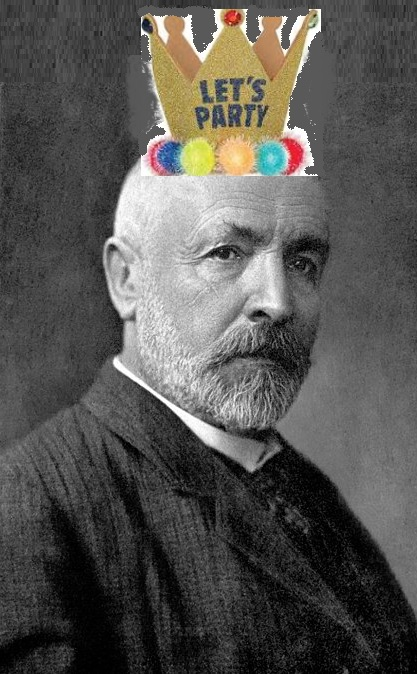
\includegraphics[height=.8\textheight]{../assets/Cantor_old}
    \end{column}
    \begin{column}{.6\textwidth}
      \begin{itemize}[<+->]
        \item Georg Cantor (1845--1918)
        \item Developed a lot of stuff this class is riding on, including cardinal and ordinal arithmetic
        %basically founded set theory! 
\item Led math into a new paradise of the infinite
\item (Or into a hellscape of epic proportions)
\item Suffered from depression, partly due to criticism of his work
\item[] (and this was before Twitter!!!)
%analogous to boltzmann in this regard and perhaps also Turing (sad that Wittgenstein bullied Turing allegedly)
%Cantor suffered his first known bout of depression in May 1884
%``This crisis led him to apply to lecture on philosophy rather than on mathematics.''
%``Cantor recovered soon thereafter, and subsequently made further important contributions, including his diagonal argument and theorem.''

%``One year later, he was outraged and agitated by a paper presented by Julius König at the Third International Congress of Mathematicians. The paper attempted to prove that the basic tenets of transfinite set theory were false. Since the paper had been read in front of his daughters and colleagues, Cantor perceived himself as having been publicly humiliated.[32] Although Ernst Zermelo demonstrated less than a day later that König's proof had failed, Cantor remained shaken, and momentarily questioning God.[13] Cantor suffered from chronic depression for the rest of his life, for which he was excused from teaching on several occasions and repeatedly confined to various sanatoria.''
      \end{itemize}
    \end{column}
  \end{columns}
\end{frame}

\begin{frame}
\frametitle{Ordering the Ordinals}
%\large

\begin{itemize}[<+->]

\item The ordinals are well-ordered by the following precedence relation:
$$\alpha <_o \beta \leftrightarrow_{\text{\emph{df}}} \alpha \in \beta$$

\item e.g. the ordinal named by $0''$ is $<_o$ the ordinal named by $0'''$ because $0'' \in 0''' = \{0, 0', 0'' \}$

\end{itemize}
\end{frame}

\begin{frame}
\frametitle{Disambiguating Two Ordering Relations}
%\large

\begin{itemize}[<+->]

\item Keep in mind that the ordinal-precedence relation $<_o$ is distinct from our notion of cardinal-precedence:

\item Where $<$ is the cardinality-ordering on sets, we have $|A| < |B|$ just in case there is an injection from $A$ to $B$ but not vice versa

\item \emph{Important fact}: $\alpha <_o \beta$ does NOT entail that $|\alpha| < |\beta|$



\end{itemize}
\end{frame}

\subsection{Ordinals as BluePrints}

\begin{frame}
\frametitle{Ordinals as Blueprints}
%\large

\begin{itemize}[<+->]

\item An ordinal can be used as a ``blueprint'' for a sequence of applications of the power set and union operations. 

\item The farther up an ordinal is in the hierarchy of ordinals, the longer the sequence, and the greater the cardinality of the end result.

\end{itemize}

Specifically, each ordinal $\alpha$ can be used to characterize the set $\mathfrak{B}_\alpha$:
\[
\mathfrak{B}_\alpha=
\begin{cases}
\mathbb{N}, \text{ if $\alpha = 0$}\\
\powerset(\mathfrak{B}_\beta), \text{ if $\alpha = \beta'$}\\
\bigcup \{\mathfrak{B}_\gamma : \gamma <_o \alpha\} \text{ if $\alpha$ is a limit ordinal (other than 0)}
\end{cases}
\]

\end{frame}

\begin{frame}
\frametitle{A Key Fact!}
%\large

\[
\mathfrak{B}_\alpha=
\begin{cases}
\mathbb{N}, \text{ if $\alpha = 0$}\\
\powerset(\mathfrak{B}_\beta), \text{ if $\alpha = \beta'$}\\
\bigcup \{\mathfrak{B}_\gamma : \gamma <_o \alpha\} \text{ if $\alpha$ is a limit ordinal (other than 0)}
\end{cases}
\]

\begin{itemize}[<+->]

\item Note that by Cantor's theorem, if $\alpha <_o \beta$, then $|\mathfrak{B}_\alpha| < |\mathfrak{B}_\beta|$.

\item This is a very useful fact!

\item For instance: 
\pause
$$\omega <_o (\omega \times \omega) <_o \omega^\omega$$
\pause
$$ \text{So: } |\mathfrak{B}_{\omega}| < |\mathfrak{B}_{\omega \times \omega}| < |\mathfrak{B}_{\omega^\omega}| $$

%$$\omega <_o (\omega \times \omega) <_o \omega^\omega <_o {^\omega\omega} \text{. So: } |\mathfrak{B}_{\omega}| < |\mathfrak{B}_{\omega \times \omega}| < |\mathfrak{B}_{\omega^\omega}| < |\mathfrak{B}_{^\omega\omega}|.$$


\end{itemize}
\end{frame}

\begin{frame}
\frametitle{Can you Supersize that?}
%\large

\begin{itemize}[<+->]
\item Recall the following definition: 
 \item[] \(
\mathfrak{B}_\alpha=
\begin{cases}
\mathbb{N}, \text{ if $\alpha = 0$}\\
\powerset(\mathfrak{B}_\beta), \text{ if $\alpha = \beta'$}\\
\bigcup \{\mathfrak{B}_\gamma : \gamma <_o \alpha\} \text{ if $\alpha$ is a limit ordinal greater than $0$}
\end{cases}
\)

\item Give an example of a set whose cardinality is ``much greater'' than $|\mathfrak{B}_{\omega \times \omega}|$, in the sense that there are infinitely many sizes of infinity between the set you identify and $|\mathfrak{B}_{\omega \times \omega}|$

%answer to 2019 version: One such set is $\mathfrak{B}_{(\omega \times \omega)+\omega}$, since $$|\mathfrak{B}_{\omega \times \omega}| < |\mathfrak{B}_{(\omega \times \omega)+0'}| < |\mathfrak{B}_{(\omega \times \omega)+0''}| < \dots  < |\mathfrak{B}_{(\omega \times \omega)+\omega}|$$


%\item Give an example of a set whose cardinality is ``much greater'' than $|\mathfrak{B}_{\omega^\omega}|$, in the sense that there are infinitely many sizes of infinity between the set you identify and $|\mathfrak{B}_{\omega^\omega}|$

%answer: One such set is $\mathfrak{B}_{(\omega^\omega)+\omega}$, since  $$|\mathfrak{B}_{\omega^\omega}| < |\mathfrak{B}_{(\omega^\omega)+0'}| < |\mathfrak{B}_{(\omega^\omega)+0''}| < \dots  < |\mathfrak{B}_{(\omega^\omega)+\omega}|$$


\end{itemize}
\end{frame}

% previous slide is as far as we got on Thursday 3/2/23. Note that to set up continuum hypothesis later, I could return to describing initial ordinals! and that would probably kill like half a class haha! 

\begin{frame}
\frametitle{Initial Ordinals}
%\large

\begin{itemize}[<+->]

\item \textbf{Initial ordinal}: an ordinal that precedes all other ordinals of the same cardinality.

\item e.g. $\omega$ is the first ordinal of cardinality $|\mathbb{N}|$, which we call $\beth_{0'}$ or $\beth_{1}$

\item An initial ordinal $\kappa$ can be used as proxy or representative for its own cardinality, so these ordinals are at least some of the ``cardinals''

\item If the generalized continuum hypothesis is true, then every cardinality corresponds to the cardinality of some initial ordinal 

%: $\kappa = |\kappa|$.

\end{itemize}
\end{frame}

\begin{frame}
\frametitle{The Beth Hierarchy}
%\large

\begin{itemize}[<+->]

\item $\beth_\alpha \text{ (read ``beth-alpha'') is the initial ordinal of cardinality } |\mathfrak{B}_\alpha|$.

\item  So, abusing notation and letting `$\beth_\alpha$' now denote a cardinal, we can write ``$\beth_\alpha = |\mathfrak{B}_\alpha|$''
%following is misleading unless you explain we're abusing notation: So: $\beth_\alpha =  |\mathfrak{B}_\alpha|$.
%seemingly rare instance of mathematicians or logicians abusing notation, something physicists do all the time! 

\item $\beth_0 = |\mathbb{N}|$ and $\beth_{0'} = |\powerset(\mathbb{N})|$ (so $\beth_{0'}$ is an \textbf{uncountable} ordinal, i.e. an ordinal whose cardinality is uncountable). 

\item Since the beths are \emph{ordinals}, they can be used to define sets bigger than anything we've considered so far. For instance: 

\item $\mathfrak{B}_{\beth_{0'}}$ (where viewed as a cardinal, $\beth_{0'} = |\powerset(\mathbb{N})|$)

\item $\mathfrak{B}_{\beth_{\beth_\omega}}$ (where as a cardinal, $\beth_{\beth_\omega} = |\mathfrak{B}_{\beth_{\omega}}|$)


\end{itemize}
\end{frame}



\subsection{Additional Practice Problems (or ones we skipped)}


\begin{frame}
\frametitle{One Union, under \dots Cantor}
%\large

\begin{itemize}[<+->]

\item Let $\mathscr{U} = \bigcup \set{\powerset^m(\mathbb{N}): m \in \mathbb{N}}$

\item Does  $\mathscr{U}$ contain the set $\underbrace{\{\{\ldots\{\{}_{\mbox{\scriptsize $n$ times}}118\underbrace{\}\}\ldots\}\}}_{\mbox{\scriptsize $n$ times}}$ for each $n>0$? 

%\answer{Let $n$ be an arbitrary natural number greater than 0. Then $\mathcal{P}^n(\mathbb{N})$ contains the set $\underbrace{\{\{\ldots\{\{}_{\mbox{\scriptsize $n$ times}}118\underbrace{\}\}\ldots\}\}}_{\mbox{\scriptsize $n$ times}}$. Since $\mathscr{U}$ contains every member of $\mathcal{P}^n(\mathbb{N})$, $\mathscr{U}$ must also contain  $\underbrace{\{\{\ldots\{\{}_{\mbox{\scriptsize $n$ times}}118\underbrace{\}\}\ldots\}\}}_{\mbox{\scriptsize $n$ times}}$.}


\end{itemize}
\end{frame}

\begin{frame}
\frametitle{Some Practice with Well-orderings}
%\large

\begin{itemize}[<+->]

\item Notation: distinguish phi-symbol `$\phi$' from the empty set `$\emptyset$'

\item Is $\powerset(\emptyset)$ well-ordered by $\in$?
%yes it is, trivially! 

\item Is $\powerset(\mathbb{Q})$  well-ordered by $\subseteq$?
% No, it is not even a total ordering. Note that $\powerset(\mathbb{Q})$ contains $\{ 5 \}$ and $\{ 1/2 \}$, but neither is a subset of the other.

\item What is $\powerset^3(\emptyset) := \powerset (\powerset (\powerset (\emptyset))) $? 

\end{itemize}
\end{frame}

\begin{frame}
\frametitle{Addition PLUS Multiplication???}
%\large
%both true 

\begin{enumerate}[<+->]

\item Is \((\omega \times 0'') + \omega <_o (\omega \times \omega) + 0''\)?
%True. \((\omega \times 0'') + \omega = ((\omega + \omega) + \omega)\), which is much smaller than \(\omega \times \omega\) (and therefore much smaller than \((\omega \times \omega) + 0''\).)

\item Does \(\omega \times (\omega + \omega) = (\omega \times \omega) + (\omega \times \omega)\)?
%True. \(\omega \times (\omega + \omega)\) is the result of using \((\omega + \omega)\) as a template, and filling each position with an \(\omega\)-sequence. So we get an \(\omega\)-sequence of \(\omega\)-sequences followed by an \(\omega\)-sequence of \(\omega\)-sequences. 
%Right hand side: \((\omega \times \omega) + (\omega \times \omega)\) is the result of starting with a sequence of type \((\omega \times \omega)\) (i.e. an \(\omega\)-sequence of \(\omega\)-sequences), and appending another sequence of type \((\omega \times \omega)\) (i.e. another \(\omega\)-sequence of \(\omega\)-sequences) to the right. So, again, we get an \(\omega\)-sequence of \(\omega\)-sequences followed by an \(\omega\)-sequence of \(\omega\)-sequences



%%practice with formal definiton of addition; could include if time:
%\item  \question{\(\alpha + 0' = \alpha \cup \{\alpha\}\) ($\alpha$ an ordinal)}

%\answer{True. It follows from the Construction Principle that \(\alpha \cup \{\alpha\} = \alpha'\), and it follows from the definition of addition that  \(\alpha + 0' = (\alpha + 0)' = \alpha'\). Putting the two together, \(\alpha \cup \{\alpha\} = \alpha'\) .}

\end{enumerate}
\end{frame}







\iffalse %***************************************************************************************

\begin{frame}
\frametitle{The Continuum Hypothesis}
%\large

\begin{itemize}[<+->]

\item \emph{Continuum Hypothesis}: There is no set $A$ such that \(\beth_0 < |A| < \beth_1\), where these beths denote cardinals, e.g. $\beth_1 = |\beth_1| = |\omega|$.

\item i.e. there is no set whose cardinality is between $|\mathbb{N}|$ and the cardinality of the `continuum', i.e. $|\mathcal{P}(\mathbb{N})| = |\mathbb{R}|$

\item \emphz{Generalized CH}: There is no set \(A\) such that \(\beth_\alpha < |A| < \beth_{\alpha + 1}\).

\item If true, then every cardinality corresponds to the cardinality of some initial ordinal in the Beth hierarchy of initial ordinals. 

% Note that the summary sheet has a commented out section on the Aleph hierarchy

\end{itemize}
\end{frame}


\subsection{The Burali-Forti Paradox}
% recall that I already have draft slides on this material, i think from week 0!

\begin{frame}
\frametitle{Burali--Forti `Paradox'}
%\large

\begin{itemize}[<+->]

\item We keep talking about the ordinals, but we can prove that there cannot exist a set of all ordinal numbers

\item In general, there can be no such thing as the set of all sets. Such a set would have to be a member of itself, and hence fail to contain every set.
%https://en.wikipedia.org/wiki/Absolute_Infinite

\item Of course, `set' is a technical term, so this isn't a paradox in the strict logical sense

\end{itemize}
\end{frame}

\begin{frame}
\frametitle{The BF `Paradox'}
%\large

\begin{itemize}[<+->]

\item Suppose, for \textit{reductio}, that $\Omega$ is the set of all ordinals.

\item Since $\Omega$ consists of every ordinal, it consists of every ordinal that's been introduced so far. But a new ordinal is just the set of every ordinal that's been introduced so far. So: \textbf{$\Omega$  is an ordinal}.

\item If $\Omega$ was itself an ordinal, it would be a member of itself (and therefore have itself as a predecessor). \\ But no ordinal can be its own predecessor (by irreflexivity). 
\item[] -- So: \textbf{$\Omega$  is not an ordinal} (contradicting prior bolded claim).

\item Hence, there is no set of all ordinals!

\end{itemize}
\end{frame}

\begin{frame}
\frametitle{Resolution in Zermelo's Set Theory(?)}
%\large

\begin{itemize}[<+->]

\item One way to avoid `paradox': declare it impermissible to form a set from an arbitrary property (reject ``unrestricted comprehension")

\item Axiom of separation/comprehension: it is permissible to form a set of objects that have a given property provided that they belong to a given set. 

\item i.e. any definable subclass of a set is itself a set 
%https://en.wikipedia.org/wiki/Axiom_schema_of_specification

\end{itemize}
\end{frame}

\begin{frame}
\frametitle{Some Worries about this Resolution}
%\large

\begin{itemize}[<+->]

\item But if a class of individuals exists, why can't we in general form a \textit{set}??? If there is no set, might we worry that some of the individuals in fact do not exist?

\item Does it start to feel like we are playing a game rather than surveying Platonic space?

\item Alternatively, given that our meta-language contains predicates that refer to classes that are not sets within our theory, might we worry that our theory is \textit{missing something}?

% Our metalanguage contains predicates that do not refer to any sets within the theory 
%https://en.wikipedia.org/wiki/Absolute_Infinite

\end{itemize}
\end{frame}

\begin{frame}
\frametitle{Proper Classes}
%\large

\begin{itemize}[<+->]

\item Some alternative formulations of set theory make explicit the notion of a `proper class'

\end{itemize}
\end{frame}


\subsection{\phantom{v} Connections to the Axiom of Choice}

% % Plausibly save this for the week we discuss AoC and Banach Tarksi!!!

\begin{frame}
\frametitle{Well-Ordering Theorem}
%\large

\begin{itemize}[<+->]

\item \emph{Well-ordering theorem} (Zermelo's theorem): every set can be well-ordered, i.e. equipped with a strict total order such that every non-empty subset has a smallest element

\item Perhaps surprisingly, this theorem is logically equivalent to the Axiom of Choice (AoC) \\ (in first-order logic; in 2nd-order logic the AoC is weaker)
\item[] (indeed, Zermelo originally used the AoC to prove this theorem, taking the AoC to be `obvious.')

\item Can you conceptualize or visualize a well-ordering of $\mathbb{R}$? 

\end{itemize}
\end{frame}

\begin{frame}
\frametitle{Another Logically Equivalent Theorem}
%\large

\begin{itemize}[<+->]

\item Both the well-ordering theorem and the Axiom of Choice are logically equivalent to Zorn's lemma

\item \emph{Zorn's lemma}: given a partially ordered set that has upper bounds for every totally-ordered subset, there is necessarily at least one maximal element (i.e. an element that is not smaller than any other element)

\item Used to show a number of key results in 20th century math: \\ -- every vector space has a basis; \\  every product of compact spaces is compact (Tychonoff); \\ Hahn--Banach theorem in functional analysis (can extend bounded linear functionals from a subspace to the whole space), etc. 

\item So rejecting AoC comes at great cost! 

%\item Utility of Zorn's lemma: rather than undertake a new transfinite induction, you can check the conditions of Zorn's lemma! 

\end{itemize}
\end{frame}

\begin{frame}
\frametitle{Clarifying the Equivalence}
%\large

\begin{itemize}[<+->]

\item These three claims (Axiom of Choice, well-ordering theorem, and Zorn's lemma) are logically equivalent in the following sense:

\item Working within Zermelo--Fraenkel set theory, given one of these claims, you can prove the other two.

\end{itemize}
\end{frame}

\begin{frame}
\frametitle{Axiom of Dependent Choice (DC)}
%\large

\begin{itemize}[<+->]

\item This is a weakening of the Axiom of Choice that suffices to recover most of real analysis

%https://en.wikipedia.org/wiki/Axiom_of_dependent_choice

\item In ZF, one cannot prove the existence of a non-measurable set of real numbers using only DC


\end{itemize}
\end{frame}


\fi %**********************************************************************************************************








